\section*{Results and discussion}

\subsection*{Regression for age prediction}

The WH dataset used for continuous regression contains data from 76 healthy
subjects, ranging between 6 years and 50 years of age
\cite{yeatman2014lifespan}. SGL fit to tractometry-extracted features in these
subjects accurately predicts the age of the subjects. The model reaches a mean
absolute error of 3.6 years (Figure \ref{fig:regress-results}), which is lower
than the results of a recent study that predicted age in a large sample, based
on TBSS-extracted diffusion features \cite{Richard2018-ux}. The model weights in
this case are distributed over many different tracts and dMRI tissue properties
(Figure \ref{fig:regress-beta}) This demonstrates that SGL is not coerced to
produce overly sparse results when a more accurate model requires a dense
selection of features.


\begin{figure}[!h]
    \centering
    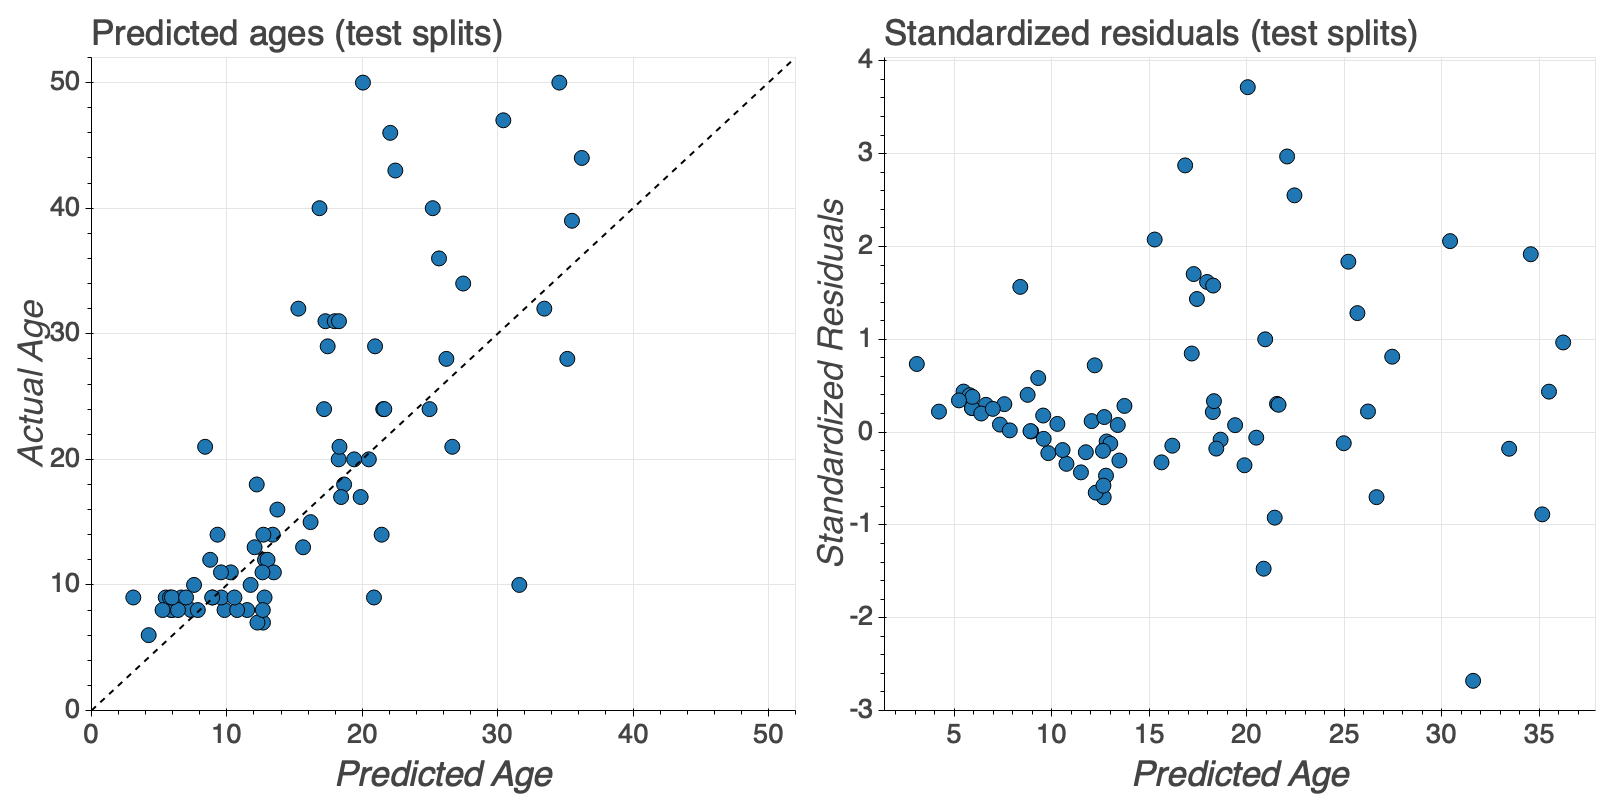
\includegraphics[width=1\textwidth]{regression_residuals.png}
    \caption{{\bf Prediction of brain age.}
    }
    \label{fig:regress-results}
\end{figure}

\begin{figure}[!h]
    \centering
    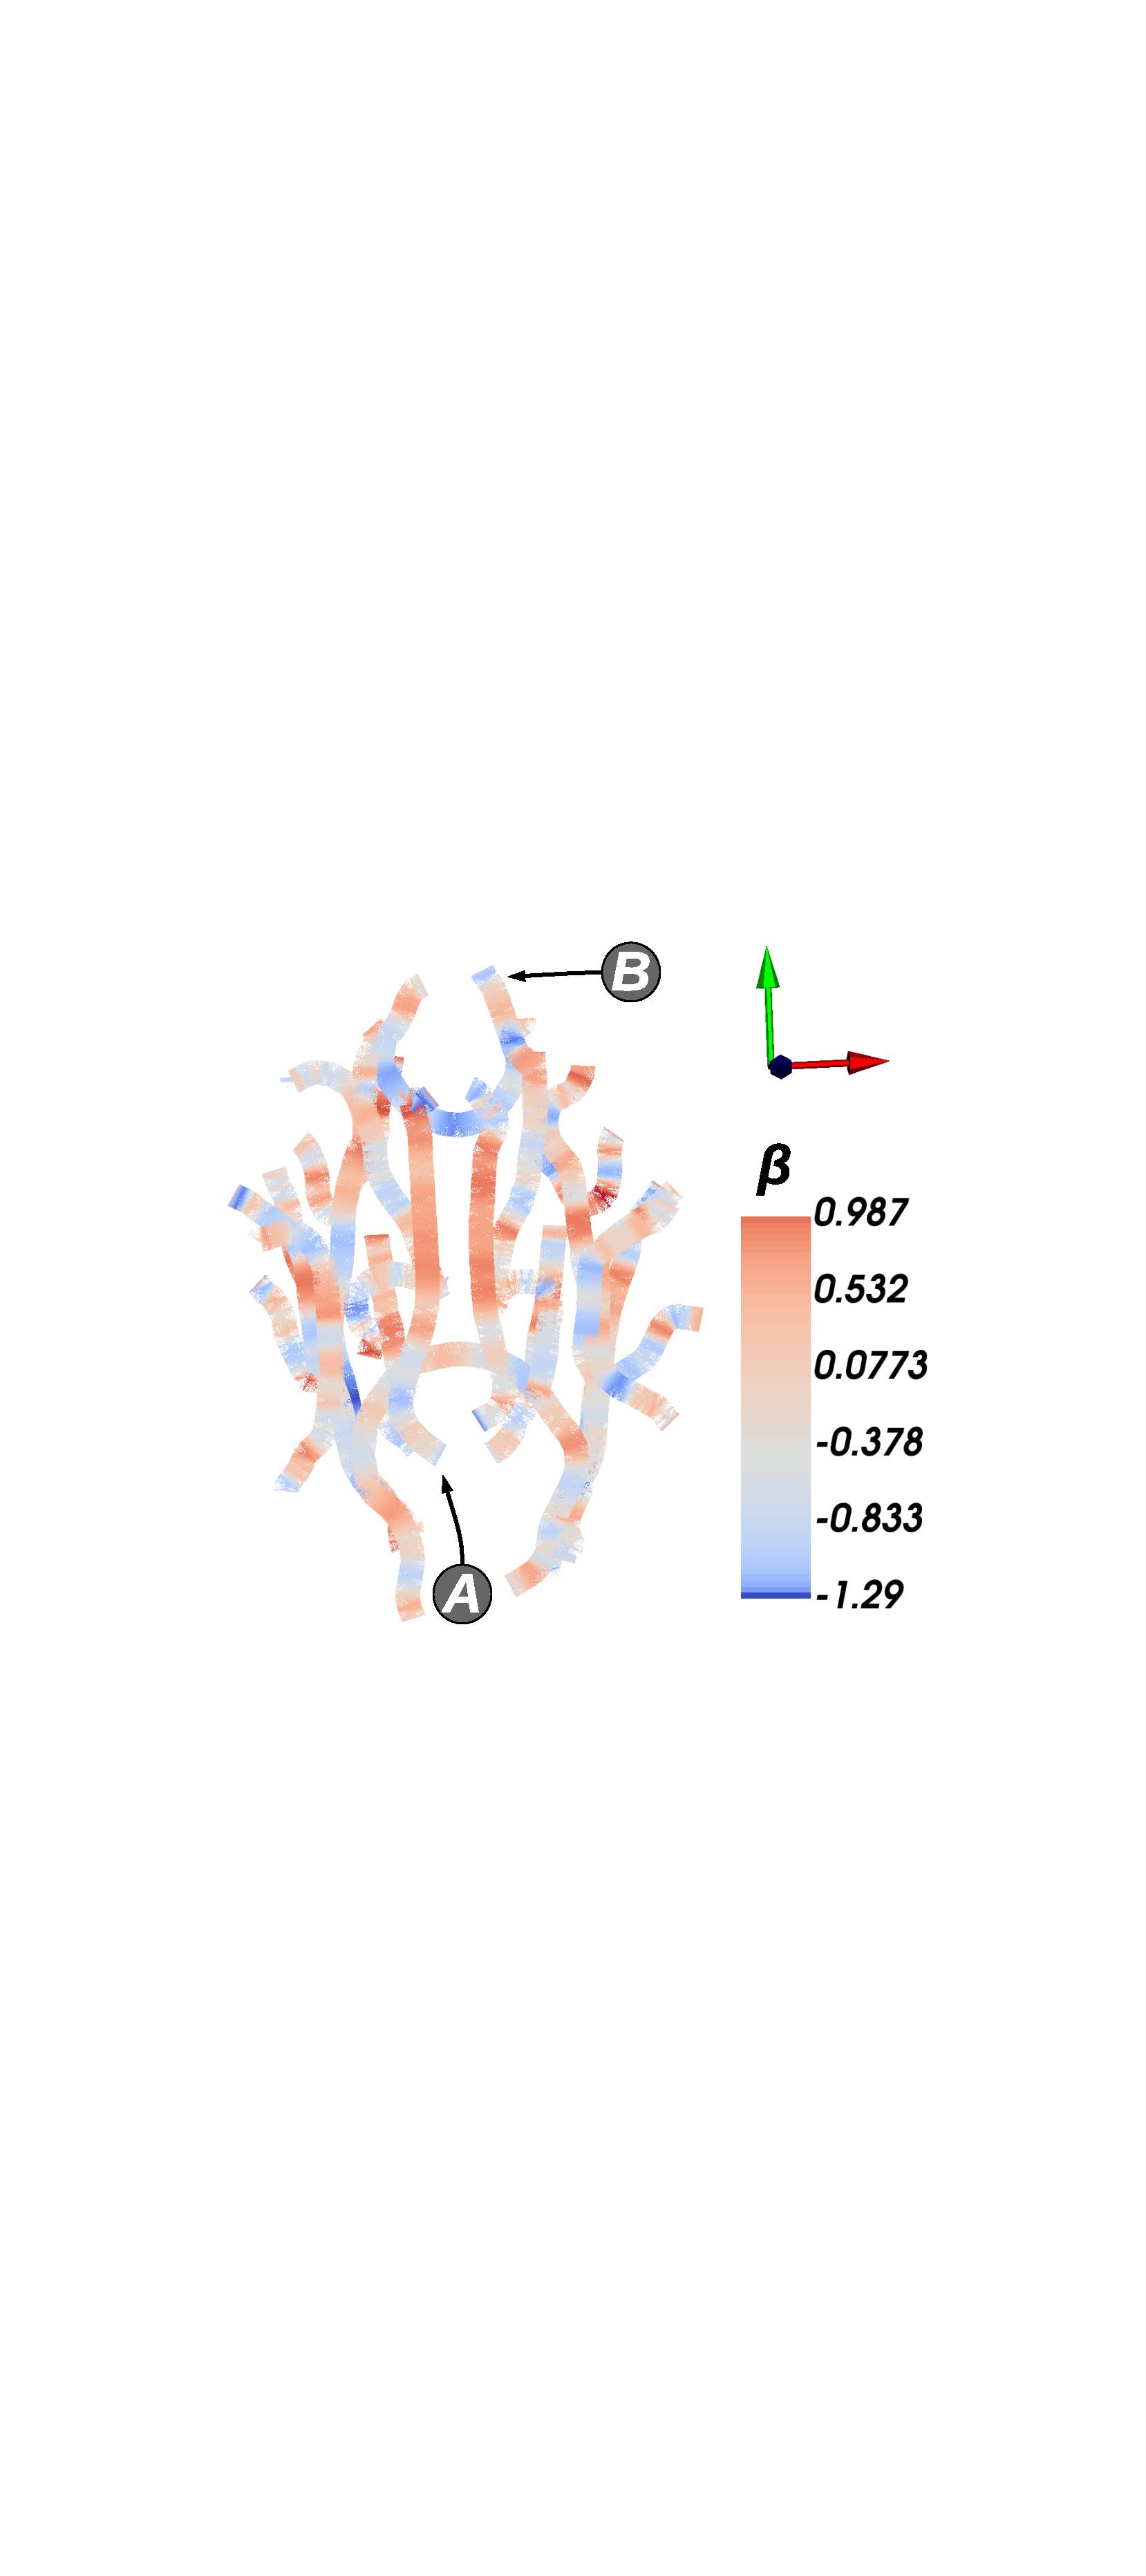
\includegraphics[width=0.5\textwidth]{regression_beta_annotated.pdf}
    \caption{{\bf Feature importance for brain age.}
    }
    \label{fig:regress-beta}
\end{figure}


\begin{figure}[!h]
    \centering
    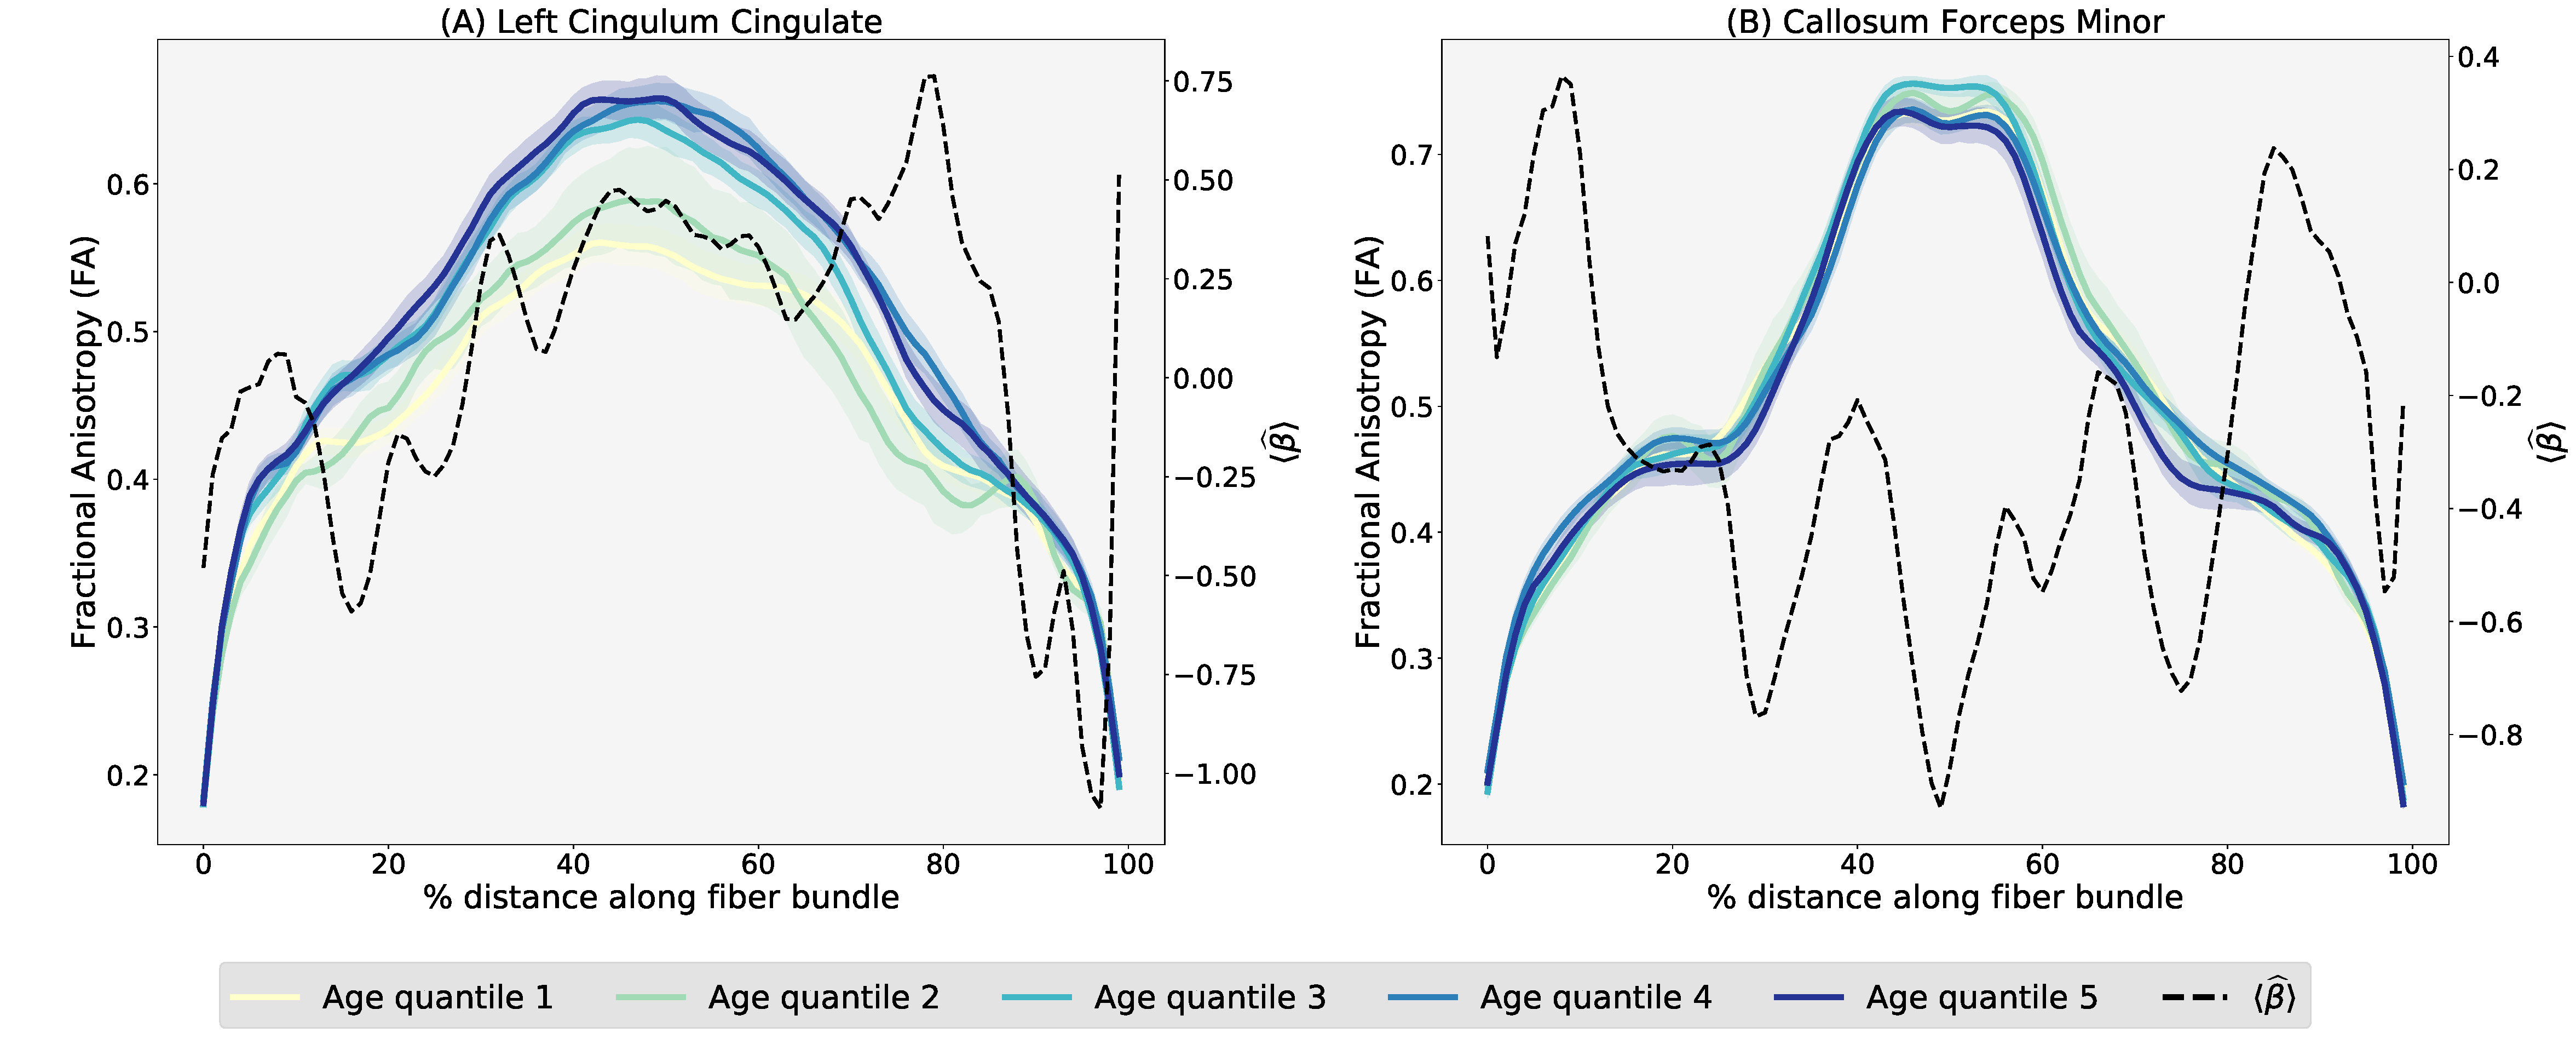
\includegraphics[width=1\textwidth]{regression_tract_profiles.pdf}
    \caption{{\bf Coefficients in context}
    It makes sense
    }
    \label{fig:regress-profiles}
\end{figure}


\begin{itemize}
  \item Regression
    \begin{itemize}
      \item Lifespan maturation age regression
      \item Insert figure showing sparsity pattern
      \item Insert figure showing weights as they relate to tract differences visible in the browser
    \end{itemize}
\end{itemize}
\begin{itemize}
  \item Failures
    \begin{itemize}
      \item Hopefully, the failures are common to both regression
        and classification so we can include them here in there own
        subsection.
      \item Insert figure demonstrating failure cases
    \end{itemize}
\end{itemize}

\subsection*{Classification for ALS detection}

Using data from a previous study of the corticospinal tract profile and
ALS\cite{sarica2017corticospinal}, we tested the performance of SGL in a
classification setting. The previous study predicted ALS status with a mean
accuracy of 80\% using a random forest algorithm based on a priori selection of
features within the corticospinal tract. SGL delivers competitive predictive
performance (mean 93\% $\pm$ 2\% accuracy, 0.978 $\pm$ 0.006 ROC AUC) without
the need for a priori feature engineering. The results of the classification
prediction are shown in Fig~\ref{fig:class-results}, with ``ground-truth'' ALS
status separated into columns, and predicted ALS status encoded by color. In
addition to this classification performance, SGL also identifies the white
matter tracts most important for ALS classification. The relative importance of
white matter features is captured in the $\beta$ coefficients from
Eq~\eqref{eq:sgl}. Fig~\ref{fig:class-beta} depicts these coefficients across
the brain, laid out on a skeleton of the major tracts. We find that SGL selects
FA metrics in the corticospinal tract and particualrly in the right
corticospinal tract as most important to ALS classification, confirming previous
findings\cite{van2011upper, toosy2003diffusion, sarica2014tractography,
sage2007quantitative, sage2009quantitative, karlsborg2004corticospinal,
ellis1999diffusion, cosottini2005diffusion, ciccarelli2009investigation,
abe2010voxel} and identifying exactly the portions of the brain that were
selected \emph{a priori} in the previous study from which we collected our
data\cite{sarica2017corticospinal}.

\begin{figure}[!h]
    \centering
    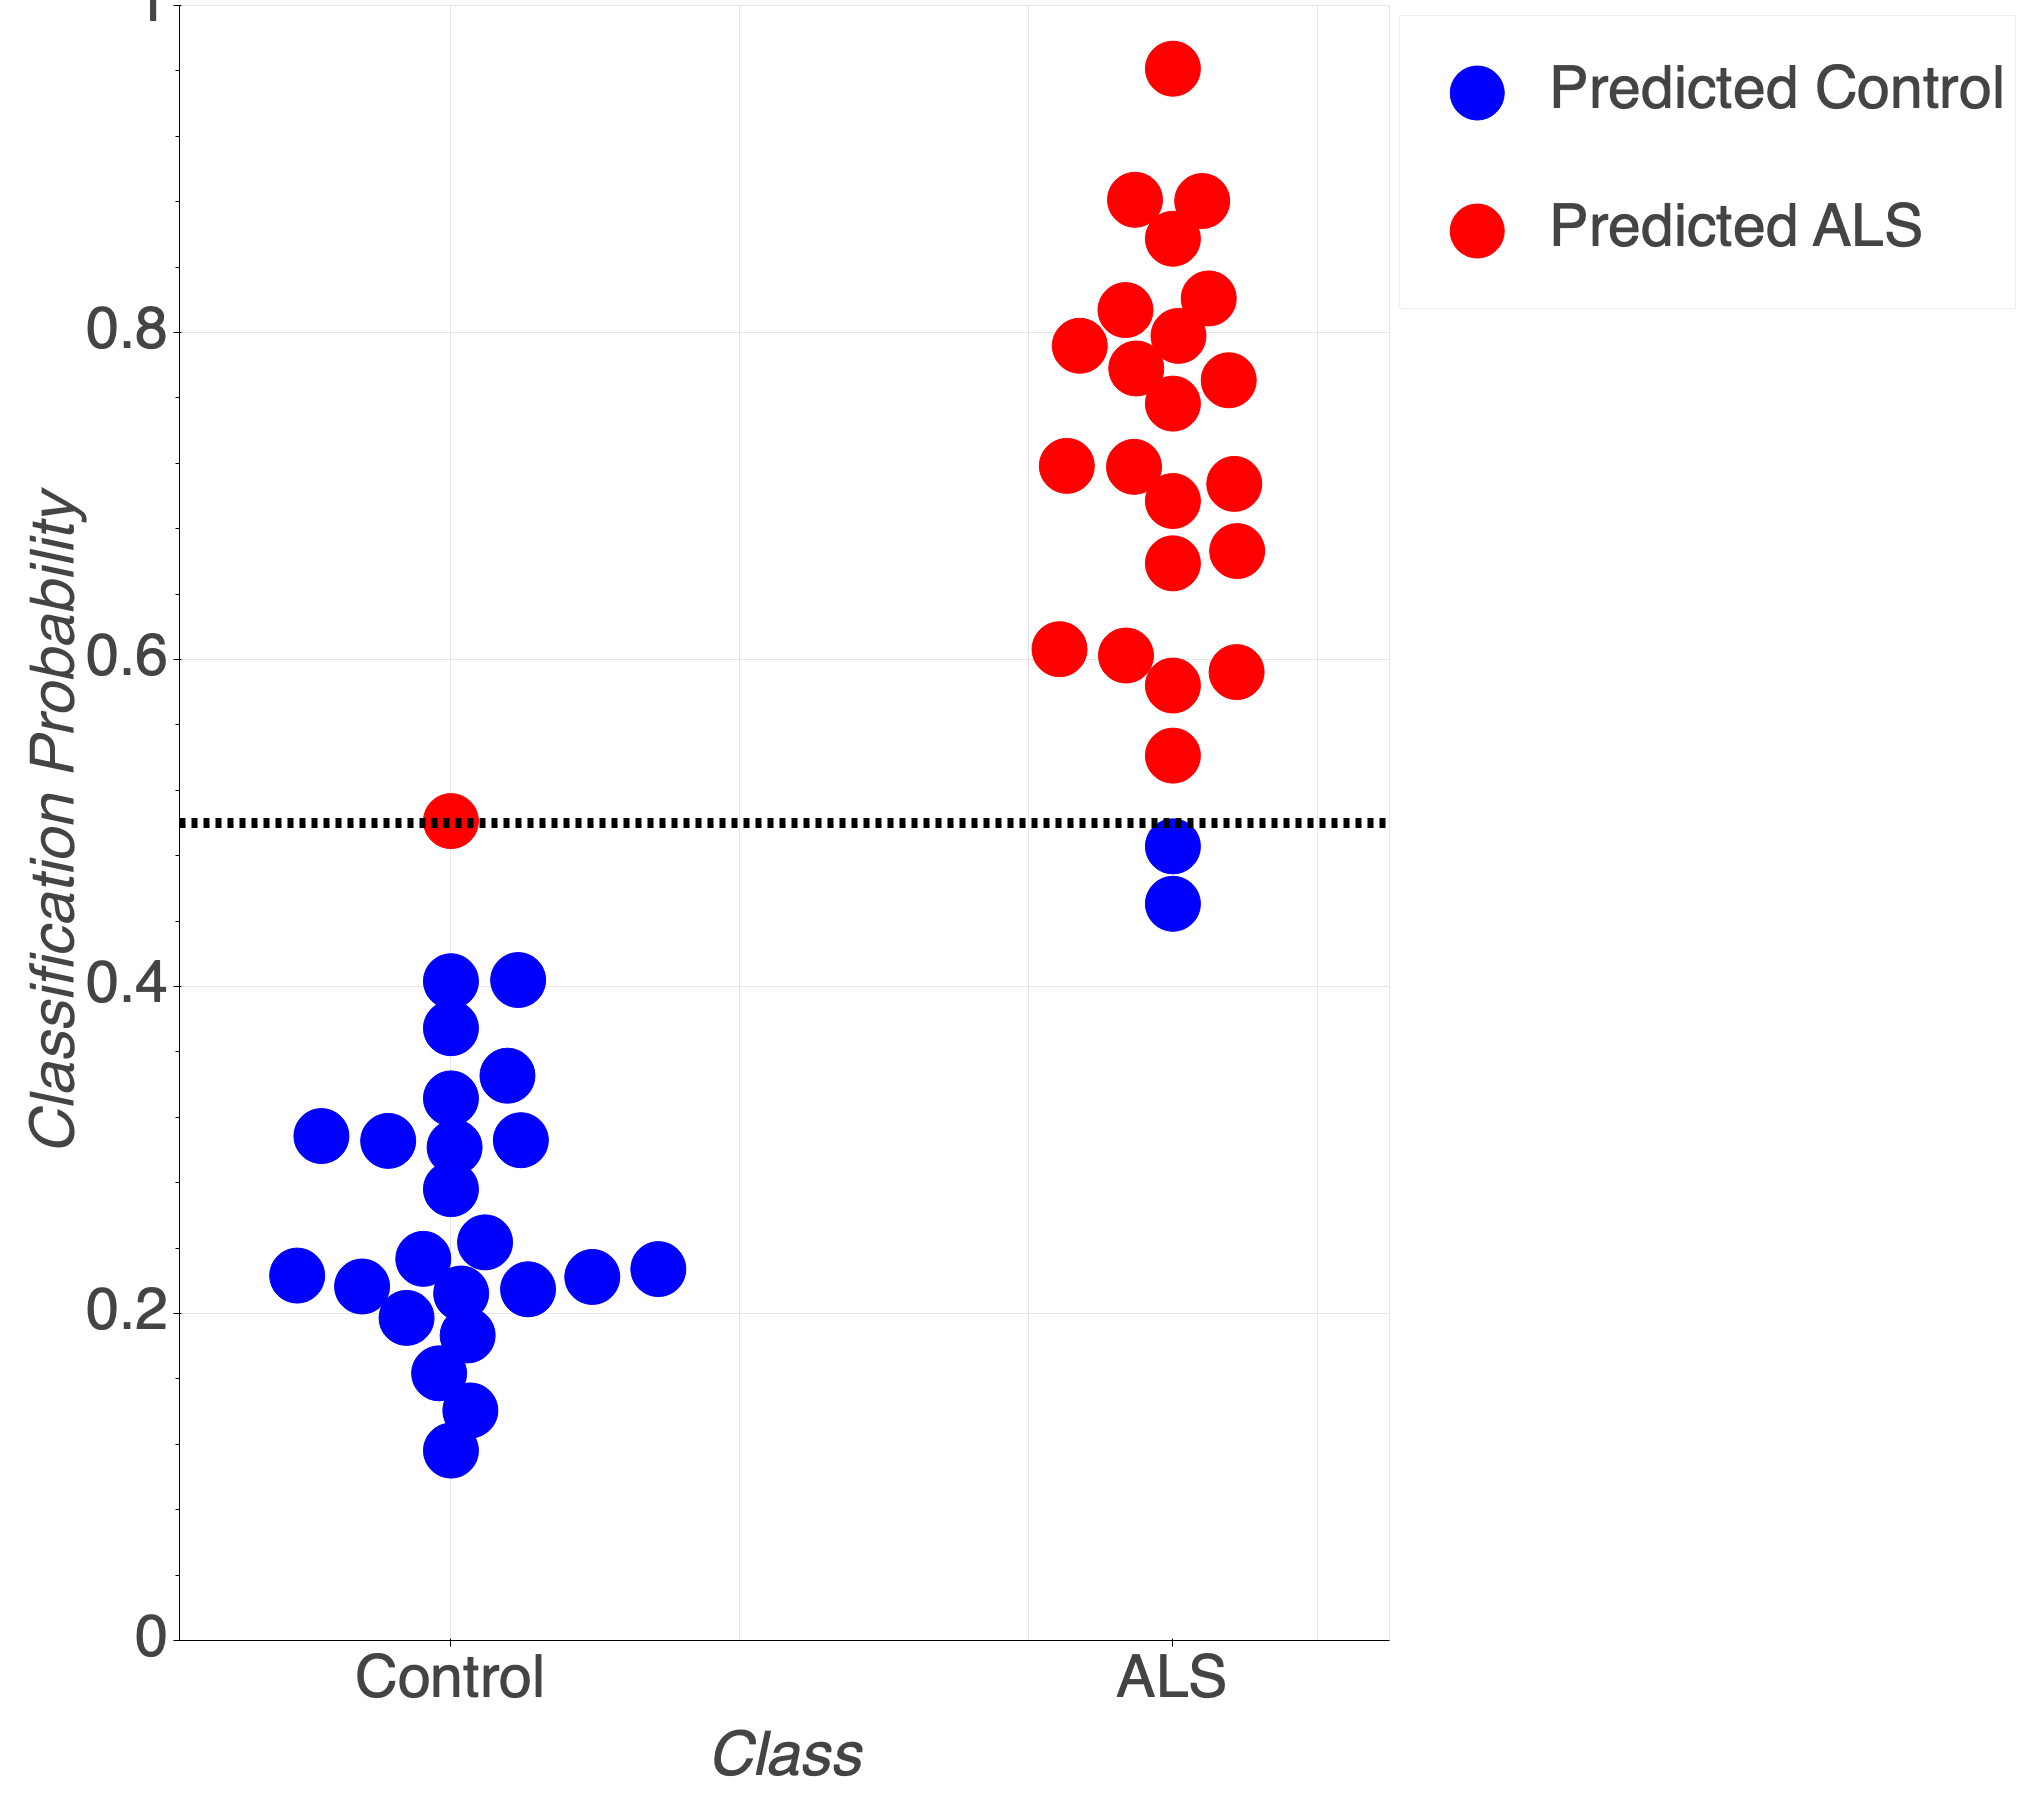
\includegraphics[width=0.65\textwidth]{classification_probs.png}
    \caption{{\bf Prediction of ALS status.}
        Classification probabilities for each subject's ALS diagnosis. Controls
        are on the left while patients are on the right. Predicted controls are in blue
        and predicted patients are in red. Thus, false positive are represented as red
        dots on the left, while false negatives are represented as blue dots on the
        right. The SGL algorithm achieves 93\% $\pm$ 2\% accuracy,with 0.978 $\pm$ 0.006
        ROC AUC}
    \label{fig:class-results}
\end{figure}

\begin{figure}[!h]
    \centering
    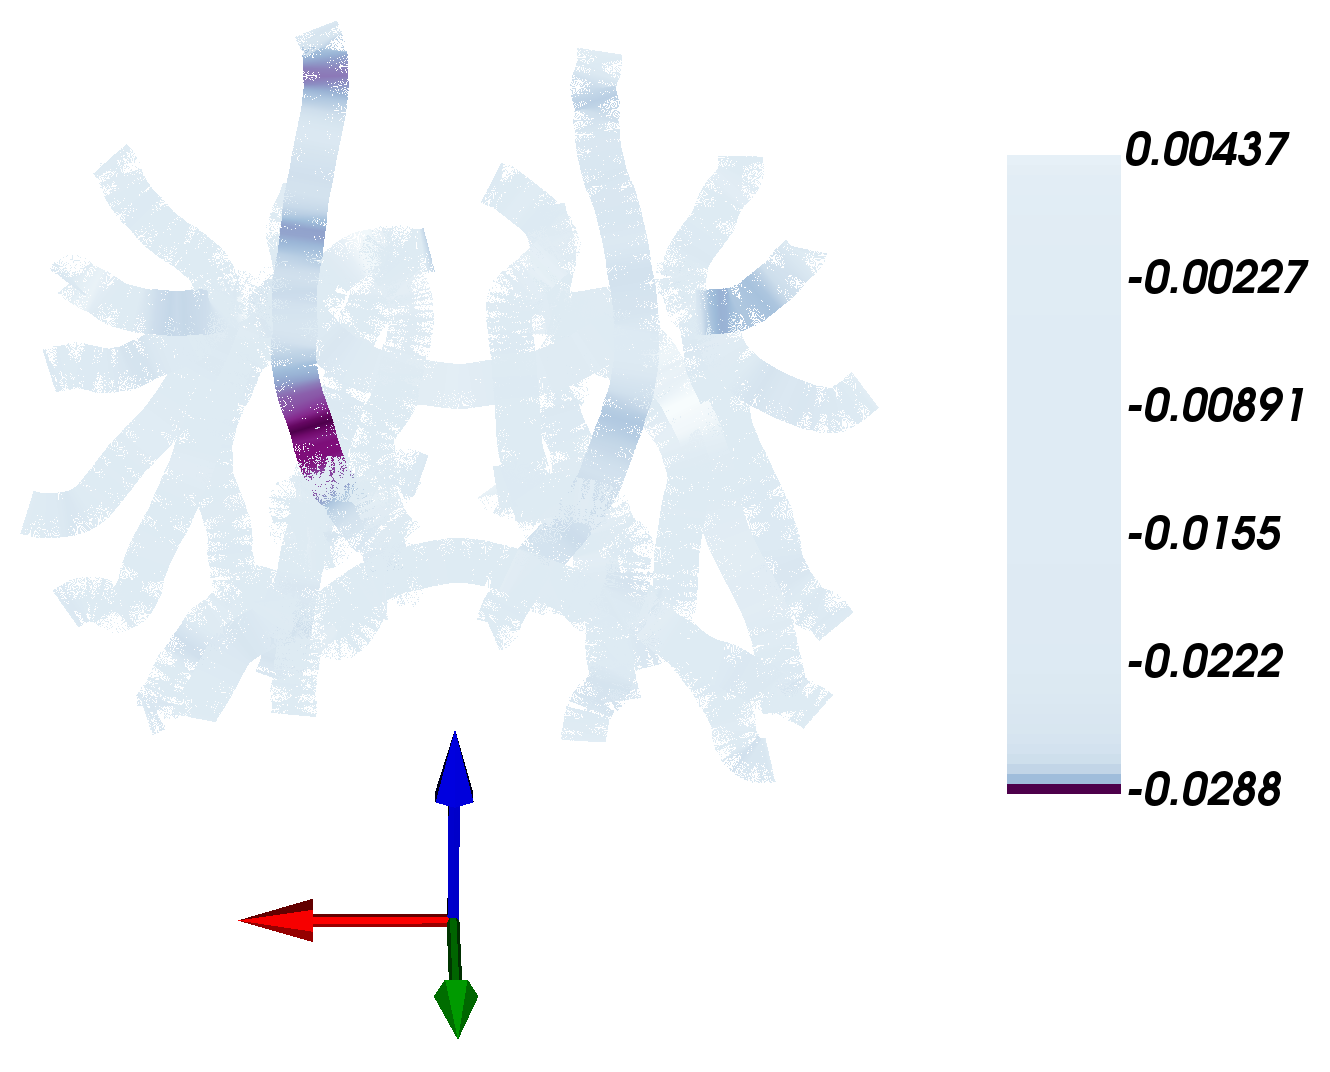
\includegraphics[width=0.95\textwidth]{classification_beta_bupu.png}
    \caption{{\bf Feature importance for prediction of ALS status.}
        SGL coefficients are presented on a skeleton of the major tracts. The
    brain is oriented with the right hemisphere to our left and anterior out of
    the page. As expected large negative coefficients are in the FA of the
    corticospinal tract (and particularly right CST, here to the left)}
    \label{fig:class-beta}
\end{figure}


\begin{figure}[!h]
    \centering
    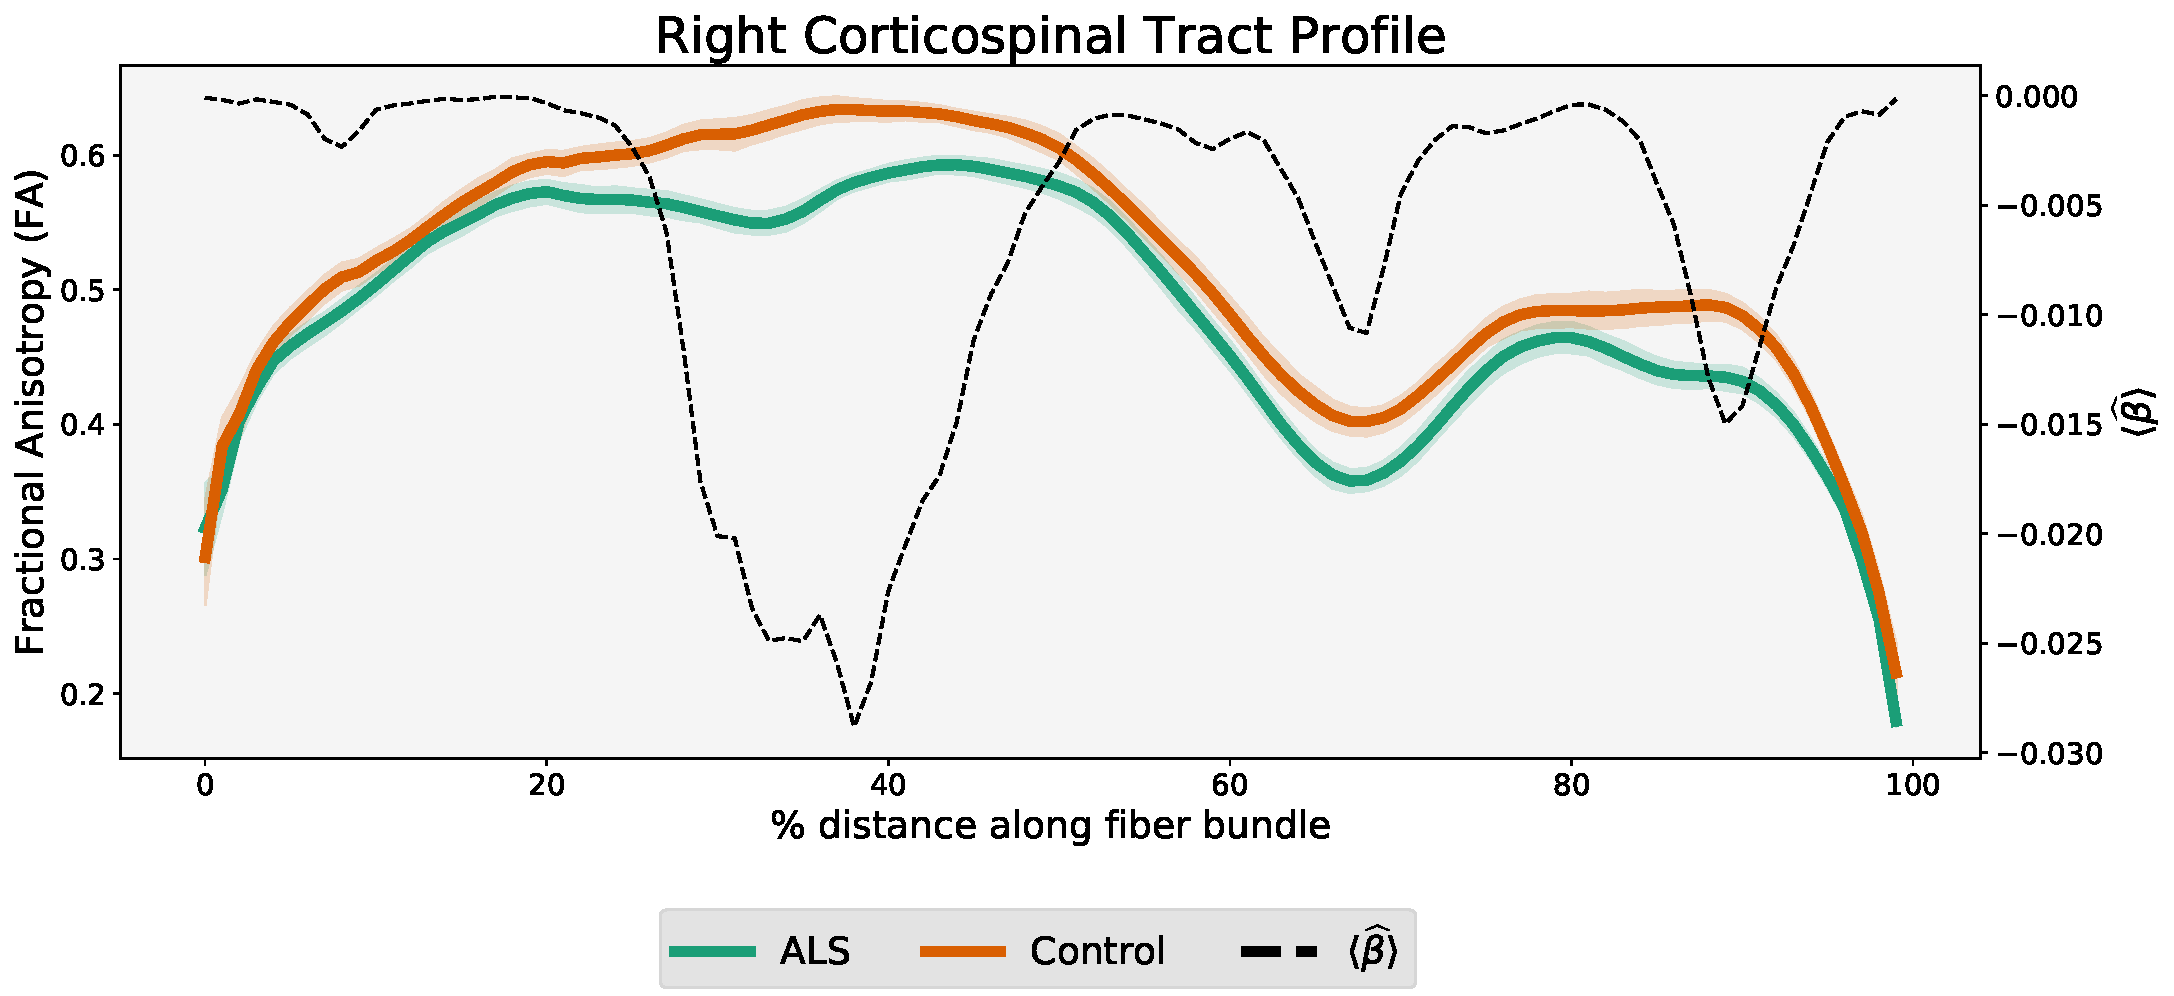
\includegraphics[width=0.95\textwidth]{classification_tract_profiles.pdf}
    \caption{{\bf Coefficients with FA tract profiles}
       }
    \label{fig:class-profiles}
\end{figure}


\begin{figure}[!h]
    \centering
    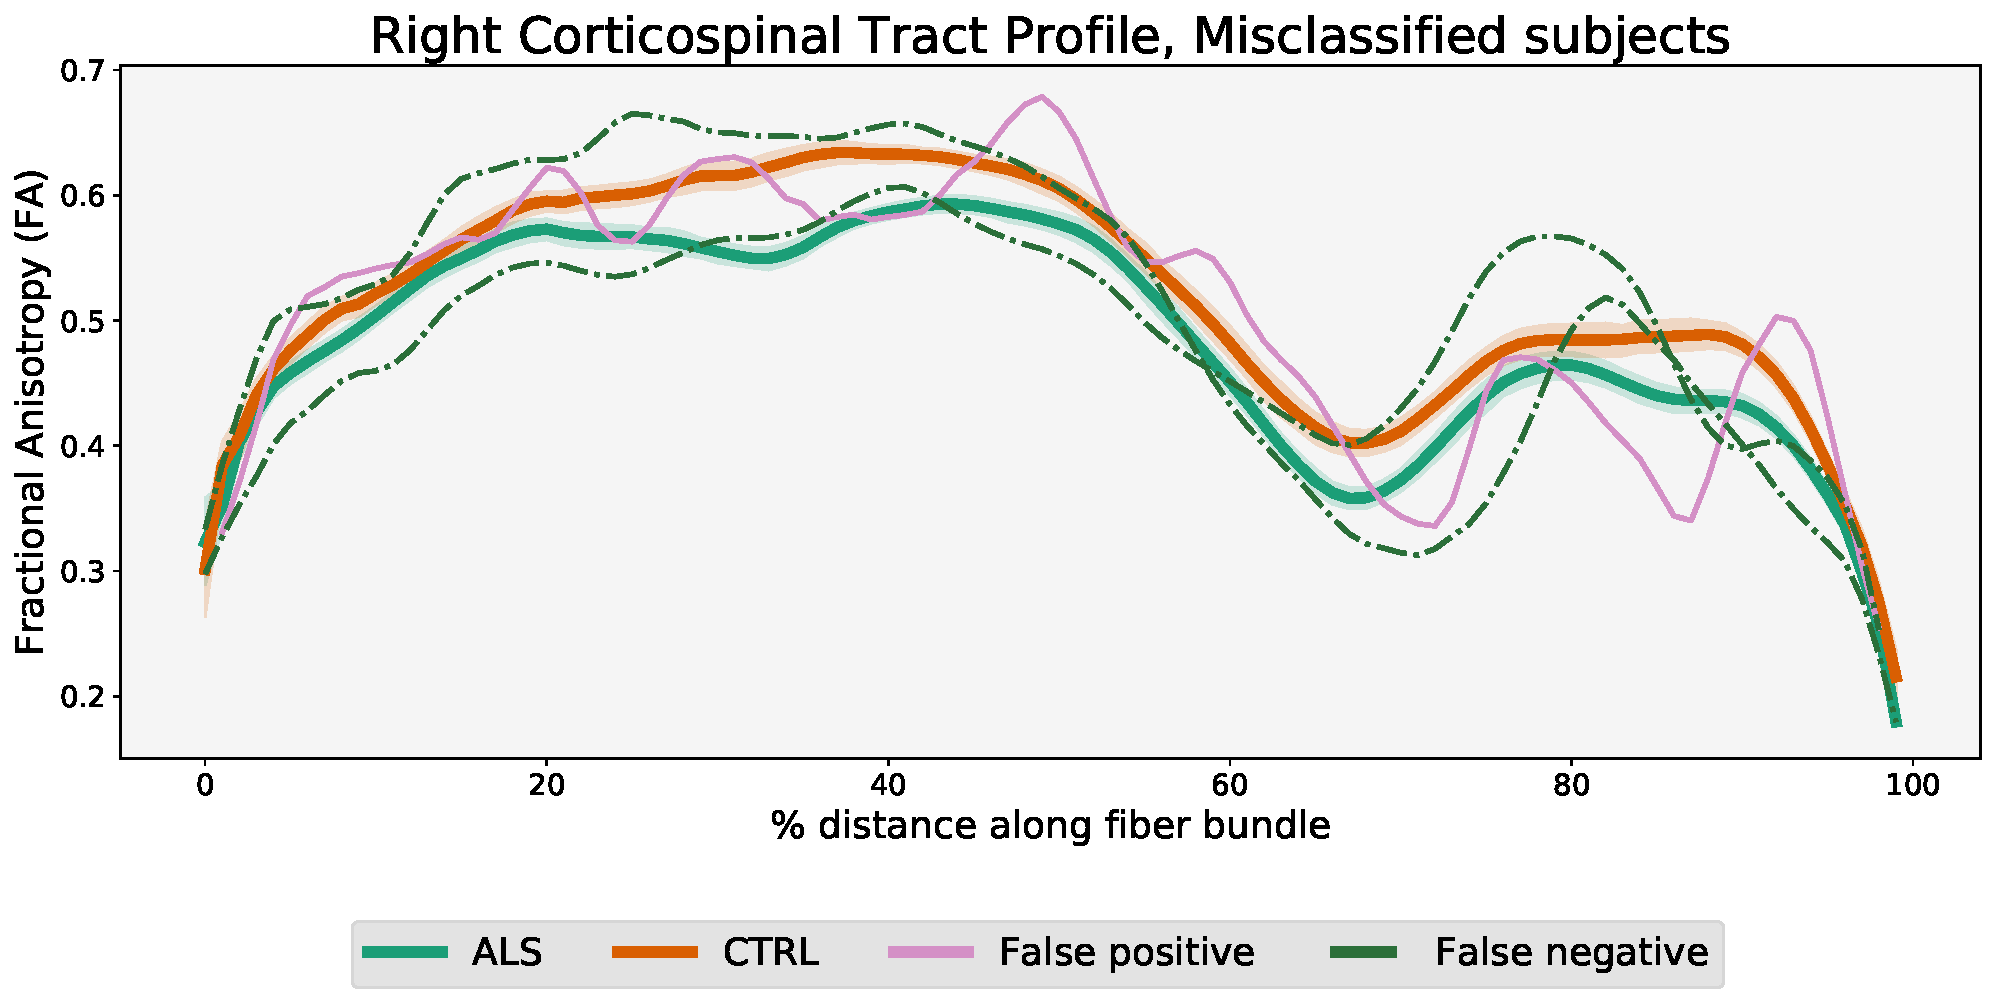
\includegraphics[width=0.95\textwidth]{classification_subjects_profiles.pdf}
    \caption{{\bf Mis-classifications}
       They make sense}
    \label{fig:class-errors}
\end{figure}


\begin{itemize}
  \item Classification
    \begin{itemize}
      \item Insert figure showing weights as they relate to tract differences visible in the browser
    \end{itemize}
\end{itemize}

